% AWS Nitro System与SRD协议技术详解
% 用于Chapter 3: 交换机设计 和 Chapter 4: 现代优化技术

\section{AWS Nitro系统：硬件卸载的虚拟化架构}

\subsection{Nitro架构演进}

AWS Nitro系统代表了云计算虚拟化架构的根本性重构。传统虚拟化架构中，Hypervisor需要消耗高达25\%的主机计算资源来处理网络、存储和安全任务。Nitro系统通过专用硬件卸载这些功能，将虚拟化开销降至接近零。

\begin{table}[htbp]
\centering
\caption{AWS Nitro系统演进历程}
\begin{tabular}{@{}llll@{}}
\toprule
\textbf{年份} & \textbf{实例} & \textbf{里程碑} & \textbf{性能} \\
\midrule
2013 & C3 & Nitro起步，网络卸载 & 10 Gbps \\
2014 & C4 & 存储卸载(EBS) & - \\
2015 & - & 收购Annapurna Labs & - \\
2017 & C5 & 完整Nitro系统 & 25 Gbps \\
2018 & - & EFA v1发布 & 100 Gbps \\
2020 & - & SRD协议引入 & 微秒级延迟 \\
2022 & - & EFA v2 + ENA Express & 200 Gbps \\
2024 & P5en & EFA v3发布 & 3.2 Tbps \\
\bottomrule
\end{tabular}
\end{table}

\subsection{Nitro系统核心组件}

Nitro系统由以下专用硬件卡组成：

\begin{itemize}
    \item \textbf{Nitro Controller}: 资源分配、实例生命周期管理、控制平面通信
    \item \textbf{Nitro Networking}: VPC数据平面卸载、ENA/EFA网络接口、安全组执行
    \item \textbf{Nitro Storage}: NVMe接口暴露、EBS数据平面、本地存储管理
    \item \textbf{Nitro Security}: 硬件可信根、安全启动验证、加密卸载
\end{itemize}

\begin{figure}[htbp]
\centering
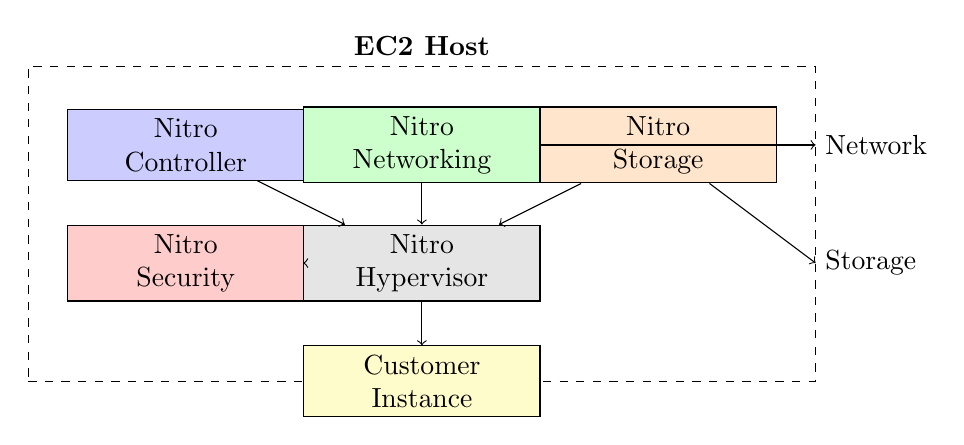
\begin{tikzpicture}[
    box/.style={rectangle, draw, minimum width=3cm, minimum height=0.8cm, align=center},
    bigbox/.style={rectangle, draw, dashed, minimum width=10cm, minimum height=4cm}
]
% EC2 Host
\node[bigbox] (host) at (0,0) {};
\node[above] at (host.north) {\textbf{EC2 Host}};

% Nitro Cards
\node[box, fill=blue!20] (ctrl) at (-3,1) {Nitro\\Controller};
\node[box, fill=green!20] (net) at (0,1) {Nitro\\Networking};
\node[box, fill=orange!20] (stor) at (3,1) {Nitro\\Storage};
\node[box, fill=red!20] (sec) at (-3,-0.5) {Nitro\\Security};

% Hypervisor
\node[box, fill=gray!20] (hyp) at (0,-0.5) {Nitro\\Hypervisor};

% Instance
\node[box, fill=yellow!20] (inst) at (0,-2) {Customer\\Instance};

% Connections
\draw[->] (ctrl) -- (hyp);
\draw[->] (net) -- (hyp);
\draw[->] (stor) -- (hyp);
\draw[->] (sec) -- (hyp);
\draw[->] (hyp) -- (inst);

% External
\node[right] at (5,1) {Network};
\draw[->] (net) -- (5,1);
\node[right] at (5,-0.5) {Storage};
\draw[->] (stor) -- (5,-0.5);
\end{tikzpicture}
\caption{AWS Nitro系统架构}
\end{figure}

\subsection{网络性能优化机制}

\subsubsection{单流带宽规格}

AWS Nitro网络针对不同类型的流量提供差异化的带宽保证：

\begin{table}[htbp]
\centering
\caption{Nitro网络单流带宽规格}
\begin{tabular}{@{}lll@{}}
\toprule
\textbf{流类型} & \textbf{带宽} & \textbf{适用场景} \\
\midrule
外部/默认流 & 5 Gbps & 互联网、跨区域 \\
Cluster Placement Group & 10 Gbps (TCP) / 8 Gbps (UDP) & 同AZ物理邻近 \\
ENA Express & 25 Gbps & 同AZ内基于SRD \\
EFA & 最高3.2 Tbps & HPC/ML工作负载 \\
\bottomrule
\end{tabular}
\end{table}

\subsubsection{数据包处理加速路径}

Nitro Card实现了连接状态缓存机制：

\begin{enumerate}
    \item \textbf{首包处理}：完整的安全组、路由、ACL检查，建立连接状态
    \item \textbf{后续包处理}：直接查询缓存的连接状态，走加速路径
    \item \textbf{Conntrack缓存}：Nitro Card维护每个流的连接跟踪表
\end{enumerate}

首包由于需要建立状态，延迟较高；后续包通过状态缓存实现低延迟转发。

\section{SRD协议：可扩展可靠数据报}

\subsection{SRD设计哲学}

SRD (Scalable Reliable Datagram) 是AWS为数据中心网络设计的专有传输协议，其核心创新在于：

\begin{itemize}
    \item \textbf{可靠但乱序传输}：保证数据可靠到达，但不保证顺序
    \item \textbf{应用层排序}：将顺序控制交给应用层，避免队头阻塞
    \item \textbf{消息为中心}：提供消息级别的网络抽象
\end{itemize}

\subsection{SRD四大核心技术}

\begin{enumerate}
    \item \textbf{智能多路径传输}
    \begin{itemize}
        \item 单流分布在最多64条并行路径
        \item 充分利用Clos网络的多路径特性
        \item 自动检测和避让拥塞路径
    \end{itemize}
    
    \item \textbf{微秒级重传}
    \begin{itemize}
        \item Nitro Card硬件实现重传
        \item 重传延迟从毫秒级降至微秒级
        \item 亚毫秒级拥塞控制响应
    \end{itemize}
    
    \item \textbf{数据包级拥塞控制}
    \begin{itemize}
        \item 实时检测路径拥塞
        \item 动态迁移流量到空闲路径
        \item 避免热点和Incast问题
    \end{itemize}
    
    \item \textbf{硬件完全卸载}
    \begin{itemize}
        \item 所有SRD处理在Nitro Card完成
        \item 不占用主机CPU资源
        \item 透明支持TCP/UDP应用
    \end{itemize}
\end{enumerate}

\subsection{SRD vs 传统协议对比}

\begin{table}[htbp]
\centering
\caption{传输协议技术对比}
\begin{tabular}{@{}lcccc@{}}
\toprule
\textbf{协议} & \textbf{可靠性} & \textbf{多路径} & \textbf{延迟} & \textbf{部署复杂度} \\
\midrule
TCP & 可靠有序 & 单路径 & 毫秒级 & 软件实现 \\
UDP & 无保证 & 应用决定 & 微秒级 & 简单 \\
InfiniBand RC & 可靠有序 & 硬件多路径 & 微秒级 & 需专用HCA \\
RoCE v2 & 依赖网络层 & 硬件多路径 & 微秒级 & 需无损以太网 \\
\textbf{SRD} & \textbf{可靠乱序} & \textbf{64路径} & \textbf{微秒级} & \textbf{需Nitro} \\
Falcon & 可靠传输 & 硬件多路径 & 微秒级 & 需Intel IPU \\
\bottomrule
\end{tabular}
\end{table}

\subsection{SRD三大应用场景}

\subsubsection{场景1: EFA (HPC/ML专用加速)}

EFA (Elastic Fabric Adapter)是SRD技术的首个主要战场：

\textbf{HPC应用性能}：
\begin{itemize}
    \item 计算流体动力学(CFD)：扩展到数千核心，性能媲美InfiniBand集群
    \item 天气预报模型：支持更细网格、更精确预报
    \item 基因组计算：显著减少序列比对和组装时间
\end{itemize}

\textbf{ML训练改进}：
\begin{itemize}
    \item 端点延迟降低30\%
    \item 小消息Allreduce性能提升50\%
    \item PyTorch FSDP训练性能提升18\%
    \item Megatron-LM性能提升8\%
\end{itemize}

\subsubsection{场景2: EBS io2 Block Express (存储加速)}

SRD集成到EBS最高性能卷类型：
\begin{itemize}
    \item 延迟改善：2.5-3.5倍降低
    \item 一致性亚毫秒I/O响应
    \item 客户案例：SQL查询时间减少30\%，TPS提升20\%
\end{itemize}

\subsubsection{场景3: ENA Express (通用网络加速)}

2022年发布的ENA Express实现了SRD技术的民主化：

\textbf{透明性特征}：
\begin{itemize}
    \item 无需修改应用代码
    \item 无需安装特殊驱动
    \item API/控制台一键开启
    \item 所有TCP/UDP自动走SRD
\end{itemize}

\textbf{性能提升}：
\begin{itemize}
    \item P99.9延迟降低85\%
    \item 单TCP流带宽：5 Gbps $\rightarrow$ 25 Gbps
\end{itemize}

\textbf{适用工作负载}：文件系统、内存数据库、媒体编码、大数据分析、微服务架构

\section{EFA演进与AI基础设施}

\subsection{EFA三代演进}

\begin{table}[htbp]
\centering
\caption{EFA架构演进}
\begin{tabular}{@{}llll@{}}
\toprule
\textbf{版本} & \textbf{年份} & \textbf{带宽} & \textbf{关键特性} \\
\midrule
EFA v1 & 2018 & 100 Gbps & OS bypass, MPI/NCCL支持 \\
EFA v2 & 2022 & 200 Gbps & 延迟降低30\% \\
EFA v3 & 2024 & 3.2 Tbps & H200 GPU, 延迟降低35\% \\
\bottomrule
\end{tabular}
\end{table}

\subsection{EFA-only接口 (2024年10月)}

\textbf{背景问题}：
\begin{itemize}
    \item 传统EFA耦合ENA设备，消耗IP地址
    \item AI/ML规模扩大时IPv4地址空间受限
    \item Linux多接口路由挑战（源IP不匹配）
\end{itemize}

\textbf{解决方案}：
\begin{itemize}
    \item EFA-only接口：仅EFA设备，无ENA设备
    \item 使用SRD协议通过MAC地址通信
    \item 不分配IP地址，解决扩展性问题
\end{itemize}

\textbf{使用限制}：
\begin{itemize}
    \item 只能作为辅助接口
    \item 主接口必须是EFA+ENA或纯ENA（用于TCP/IP路由）
\end{itemize}

\subsection{Trainium芯片与UltraServers}

\subsubsection{Trainium2技术规格}

\begin{table}[htbp]
\centering
\caption{Trainium2与Trn2实例规格}
\begin{tabular}{@{}ll@{}}
\toprule
\textbf{组件} & \textbf{规格} \\
\midrule
单芯片算力 & 万亿次计算/秒 \\
单芯片内存 & 96GB HBM3e \\
单芯片引擎 & 8×NeuronCore-V3 \\
Trn2芯片数 & 16个Trainium2 \\
Trn2算力 & 20.8 FP8 petaflops \\
Trn2内存 & 1.5TB HBM，46TB/s带宽 \\
Trn2网络 & 3.2Tbps EFA \\
价格性能 & 比GPU实例好30-40\% \\
\bottomrule
\end{tabular}
\end{table}

\subsubsection{Trn2 UltraServers}

UltraServers是AWS为超大规模模型训练推出的全新EC2产品：

\begin{itemize}
    \item \textbf{架构}：4个Trn2服务器合并为一个单元
    \item \textbf{芯片}：64个Trainium2芯片
    \item \textbf{互联}：NeuronLink超高速互连（蓝色线缆标识）
    \item \textbf{算力}：83.2 FP8 petaflops
    \item \textbf{内存}：6TB HBM，185TB/s总带宽
    \item \textbf{网络}：12.8Tbps EFA
\end{itemize}

\textbf{优势}：
\begin{itemize}
    \item 推理：业界领先的响应时间，最佳实时体验
    \item 训练：更快的集体通信，提升模型并行效率
\end{itemize}

\subsubsection{Project Rainier}

AWS与Anthropic合作打造的超大规模AI训练集群：

\begin{itemize}
    \item \textbf{规模}：近50万Trainium2芯片
    \item \textbf{部署}：跨多个美国数据中心
    \item \textbf{时间}：2024年12月宣布，12个月内完成部署
    \item \textbf{扩展}：预计2025年底达100万+芯片
    \item \textbf{算力}：为Anthropic提供比之前多5倍的训练算力
\end{itemize}

\subsubsection{Trainium3 (2025年底)}

AWS下一代AI芯片：

\begin{itemize}
    \item \textbf{工艺}：3nm（AWS首个3nm芯片）
    \item \textbf{算力}：2.52 PFLOPS FP8/芯片
    \item \textbf{内存}：144GB HBM3e（比Trainium2多1.5倍）
    \item \textbf{带宽}：4.9TB/s（高1.7倍）
    \item \textbf{UltraServer}：144芯片，362 FP8 PFLOPS
    \item \textbf{性能}：比Trn2 UltraServer高4.4倍
    \item \textbf{能效}：提升4倍以上
\end{itemize}

\section{云厂商网络架构对比}

\subsection{L1-L7技术栈对比}

\begin{table}[htbp]
\centering
\caption{云厂商数据中心网络技术栈对比}
\begin{tabular}{@{}lccc@{}}
\toprule
\textbf{OSI层} & \textbf{AWS} & \textbf{Google Cloud} & \textbf{Azure} \\
\midrule
L7应用 & EFA API & Cloud RDMA API & IB Verbs API \\
L6表示 & Nitro编码 & ALTS加密 & Azure Boost编码 \\
L5会话 & Nitro会话 & gRPC RPC & MANA会话 \\
\textbf{L4传输} & \textbf{SRD} & \textbf{Falcon} & \textbf{RoCE v2/IB} \\
L3网络 & VPC+ENA Express & Andromeda 2.1 & AccelNet/MANA \\
L2链路 & 以太网 & 以太网 & 以太网/IB \\
L1物理 & QSFP-DD+PAM4 & 光纤+OCS & 光纤+PAM4/HCF \\
\textbf{硬件} & \textbf{Nitro v5 DPU} & \textbf{Intel IPU E2000} & \textbf{Azure Boost} \\
\bottomrule
\end{tabular}
\end{table}

\subsection{技术路线差异}

\begin{itemize}
    \item \textbf{AWS}：专有SRD协议 + 标准以太网 + Nitro DPU硬件卸载
    \item \textbf{Google Cloud}：专有Falcon协议 + Intel IPU + OCS光电路交换
    \item \textbf{Microsoft Azure}：RoCE v2/InfiniBand混合 + Azure Boost + MANA
\end{itemize}

三种路线各有优势，AWS的SRD方案在标准以太网基础设施上实现了类似InfiniBand的低延迟高性能，同时保持了与TCP/IP应用的兼容性。
